\section{Lambda Umgebung}
Ist \textbf{partielle Abbildung der variablen} in die Terme
einer Definitionsmenge \textbf{(Domain)}

\subsection{Spezielle Umgebungen}
\begin{itemize}
    \item \varepsilon ist die \textbf{leere Umgebung}
    \item Umgebungen mit genau einer Variablen sind \textbf{Bindungen}
    \begin{itemize}
        \item Schreibweise: $x \rightarrow t$, $dom(\phi) = {x}$, $\phi(x)=t$
        \item Komposition $\phi \circ \psi$ \textit{(\phi und \psi sind Umgebungen)}:
        \begin{itemize}
            \item $dom(\phi \circ \psi) = dom(\phi) \cup dom(\psi)$
            \item \[(\phi \circ \psi)(x) =
                    \begin{cases}
                        x \in dom(\phi) & \phi(x) \\
                        sonst           & \psi(x)
                    \end{cases}\]
            \item dom(\phi) ist endlich und besteht aus Bindungen $\psi_i$ \\
            $\phi = \psi_0 \circ \psi_1 \circ \psi_2 \cdots \psi_n$
        \end{itemize}
    \end{itemize}
\end{itemize}

\subsection{Auswertung}
Die Auswertung einer Variablen \textbf{t} in \phi wird geschrieben $t \downarrow \phi$

\subsubsection{Regeln}
\begin{enumerate}
    \item Variable x
    \begin{itemize}
        \item $x \downarrow \phi = \phi(x)$
        \item $x \downarrow \phi = x$ \textit{(wenn x $\notin$ dom(\phi))}
    \end{itemize}
    \item Anwendung s auf r \textbf{(rs)} \\
    sei $p = r \downarrow \phi$ und $q = s \downarrow \phi$
    \begin{itemize}
        \item wenn p die Form \lambda x.u hat so ist
        $rs \downarrow \phi = u \downarrow [q \leftarrow x] \circ \phi$
        \item Andernfalls: $rs \downarrow \phi = p \circ q$
    \end{itemize}
    \item Abstraktion \lambda x.s \\
    $\lambda x.s \downarrow \phi = \lambda z.(s \downarrow (z \leftarrow x) \circ \phi)$ \\
    Wobei $z \notin FV(s) \cup \bigcup_{y \in dom(\phi)}FV(\phi(y))$
\end{enumerate}

\subsubsection{Beispiele}
\lstset{language=Scheme,style=customstyle}
\begin{lstlisting}
(let ((a 1))
     (plus10 (let ((a 10))
                  (lambda (x) (+ a x))))
     (let ((y 5) (x 3))
          (plus10 (+ a y))))
\end{lstlisting}
\begin{figure}[h!]
    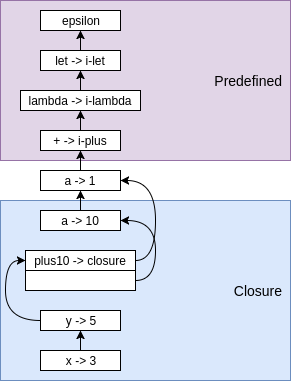
\includegraphics[scale=.5]{pics/i-environment}
    \caption{Lambda Bindings}
\end{figure}
